
\documentclass{article}

\usepackage[nonatbib, final]{neurips_2021}
\usepackage[utf8]{inputenc} % allow utf-8 input
\usepackage[T1]{fontenc}    % use 8-bit T1 fonts
\usepackage{biblatex}
\DefineBibliographyStrings{english}{andothers={\&~al\adddot}}
\addbibresource{bibliography.bib}

\usepackage{hyperref}       % hyperlinks
\usepackage{url}            % simple URL typesetting
\usepackage{booktabs}       % professional-quality tables
\usepackage{amsfonts}       % blackboard math symbols
\usepackage{nicefrac}       % compact symbols for 1/2, etc.
\usepackage{microtype}      % microtypography
\usepackage{xcolor}         % colors
\usepackage[ngerman]{babel}
\usepackage{csquotes}
\usepackage{amsmath}
\usepackage{graphicx}
\usepackage{lipsum} 

\title{SynthRAD Diffusion: Advancing Synthetic Image Generation with Conditioned Diffusion Models}


\author{
  Benedikt Arnthof\\
  Department of Statistics\\
  Ludwig-Maximilians-Universität München\\
  %Ludwigstr. 33 München \\
  \texttt{b.arnthof@campus.lmu.de} \\
}


\begin{document}
\renewcommand{\figurename}{Fig.}
\maketitle

\begin{abstract}

The source code and supplementary materials are available at {\url{https://github.com/benearnthof/SynthGenDiffusion}}
\end{abstract}

\section{Introduction}\label{intro}



\begin{figure}[h]
    \centering
    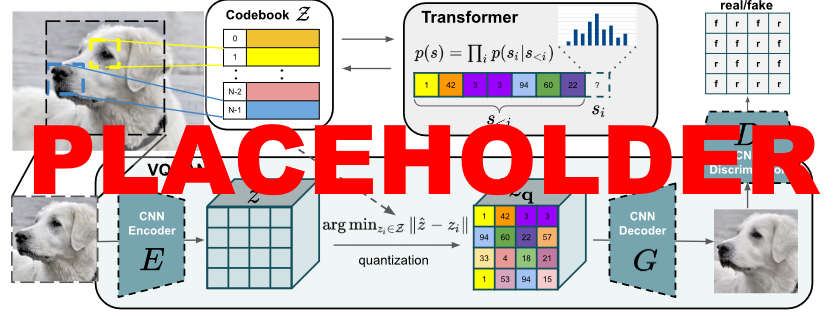
\includegraphics[width=\textwidth]{placeholder.PNG}
    \caption{}
    \label{fig:placeholder}
\end{figure}

\section{Related Work}\label{relwork}

\subsection{Medical Image Synthesis}



\section{Method}

\subsection{Background and Problem Formulation}\label{background}

\paragraph{Diffusion Models}

Diffusion Models (DMs) have emerged as the state-of-the-art not only for image modeling tasks such as super-resolution, inpainting, and image generation, but also in seemingly unrelated fields such as language models \cite{he2022diffusionbert}, or Text-to-Audio generation \cite{liu2023audioldm}. This great flexibility is owed, in equal parts, to the idea of modeling only a latent representation of the data distribution with the underlying diffusion process \cite{rombach2021highresolution}, and the generality of the model formulation itself \cite{ho2020denoising}.  
A DM repeatedly adds noise from a known distribution to the available data based on a noise schedule and uses another model, such as a U-Net, to estimate the amount of corruption introduced to the data, so that one can later use a chain of denoising steps to generate images from pure noise inputs. \\
Let $x_0$ represent an input image, where $q(x)$ represents the source distribution of all images we want to model $x \sim q(x)$. Gradually corrupting an image by sequentially adding Gaussian noise to it can then be modeled by the following process: 
\begin{equation}
    q\left(x_t \mid x_{t-1}\right)=\mathcal{N}\left(x_t ; \sqrt{1-\beta_t} \cdot x_{t-1}, \beta_t \cdot \mathbf{I}\right),
\end{equation}
where $x_1, x_2, \ldots, x_T$ represents the images at each individual noise time step $t \in T$ total time steps. Scheduling the variance of incremental noise with the hyperparameter $\beta_t \in (0, 1)$ and using the Markov property of the process we constructed in this way, we obtain \\
\begin{equation}
    q\left(x_{1: T} \mid x_0\right)=\prod_{t=1}^T q\left(x_t \mid x_{t-1}\right)
\end{equation}
as the distribution of the noisy images at every time step, conditioned on the source image $x_0$. By reparametrising $\alpha_t = 1- \beta_t$ and $\bar{\alpha}_t=\prod_{i=1}^t \alpha_i$ we obtain 
\begin{equation}
    q\left(x_t \mid x_0\right)=\mathcal{N}\left(x_t ; \sqrt{\bar{\alpha}_t} \cdot x_0,\left(1-\bar{\alpha}_t\right) \cdot \mathbf{I}\right)
\end{equation}
Where $\mathcal{N}(x;\mu,\sigma$ represents a Gaussian distribution with mean $\mu$ and variance $\sigma$. With $T \longrightarrow \infty$ $x_T$ will be corrupted completely, with pixel values from an isotropic Gaussian distribution. The Denoising Diffusion Probabilistic Model (DDPM) now performs the learned denoising task to obtain an image of the original distribution from this noise input. \\
It can now be proven that, given small enough time steps, that every individual reverse step $q(x_{t-1}|x_t$ is also Gaussian \cite{sohldickstein2015deep}. This makes it possible to train a separate neural network, such as the aforementioned U-Net, to estimate the mean $\mu_\theta(x_t, t)$ and covariance $\Sigma_\theta(x_t, t)$. With $p(x_T)$ as density function of $x_T$ we can obtain
\begin{equation}
    p_\theta\left(x_{0: T}\right)=p\left(x_T\right) \prod_{t=1}^T p_\theta\left(x_{t-1} \mid x_t\right),
\end{equation}
\begin{equation}
    p_\theta\left(x_{t-1} \mid x_t\right)=\mathcal{N}\left(x_{t-1} ; \mu_\theta\left(x_t, t\right), \Sigma_\theta\left(x_t, t\right)\right).
\end{equation}

By following results from \cite{ho2020denoising}, we see that the reverse steps are tractable, if we condition on $x_t$ and $x_0$:
\begin{equation}
q\left(x_{t-1} \mid x_t, x_0\right)=\mathcal{N}\left(x_{t-1} ; \tilde{\mu}\left(x_t, x_0\right), \tilde{\beta}_t \cdot \mathbf{I}\right)
\end{equation}

\begin{equation}\label{eq7}
    \tilde{\mu}\left(x_t, x_0\right)=\frac{\sqrt{\bar{\alpha}_{t-1}} \beta_t}{1-\bar{\alpha}_t} x_0+\frac{\sqrt{\alpha_t}\left(1-\bar{\alpha}_{t-1}\right)}{1-\bar{\alpha}_t} x_t
\end{equation}

\begin{equation}
    \tilde{\beta}_t=\frac{1-\bar{\alpha}_{t-1}}{1-\bar{\alpha}_t} \beta_t
\end{equation}

Now, given that $x_0=\frac{1}{\sqrt{\bar{\alpha}_t}}\left(x_t-\sqrt{1-\bar{\alpha}_t} \epsilon_t\right)$, where $\epsilon_t \sim \mathcal{N}(0, \mathbf{I})$ equation \ref{eq7} can be rewritten as 
\begin{equation}
    \begin{aligned}
\mu_\theta\left(x_t, t\right) & =\tilde{\mu}\left(x_t, \frac{1}{\sqrt{\bar{\alpha}_t}}\left(x_t-\sqrt{1-\bar{\alpha}_t} \epsilon_\theta\left(x_t\right)\right)\right) \\
& =\frac{1}{\sqrt{\alpha_t}}\left(x_t-\frac{1-\alpha_t}{\sqrt{1-\bar{\alpha}_t}} \epsilon_\theta\left(x_t, t\right)\right),
\end{aligned}
\end{equation}
Thus, the training objective for the noise estimation network $p_\theta$ is the optimization of the variational lower bound (VLB):
\begin{equation}
    \mathcal{L}_{V L B}=\mathcal{L}_0+\sum_{t=1}^{T-1} \mathcal{L}_t+\mathcal{L}_T
\end{equation}
\begin{equation}
    \mathcal{L}_0=-\log p_\theta\left(x_0 \mid x_1\right)
\end{equation}
\begin{equation}
    \mathcal{L}_t=K L\left(q\left(x_{t-1} \mid x_t, x_0\right) \| p_\theta\left(x_{t-1} \mid x_t\right)\right)
\end{equation}
\begin{equation}
    \mathcal{L}_T=K L\left(q\left(x_T \mid x_0\right) \| p_\theta\left(x_T\right)\right)
\end{equation}
Where $KL$ denotes the Kullback-Leibler divergence between two probability distributions, and $\mathcal{L}_T$ is simply a constant, since $x_T$ is Gaussian noise and $q(x_T|x_0)$ has no learnable parameters. To arrive at a tractable learning objective we can approximate the term $\mathcal{L_0}$ as the likelihood of a multivariate Gaussian of the form $\mathcal{N}\left(x_0 ; \mu_\theta\left(x_1, 1\right), \Sigma_\theta\left(x_1, 1\right)\right)$ which, after simplification, leads to the approximate training objective: 
\begin{equation}
    L_{\text {simple }}(\theta):=\mathbb{E}_{t, \mathbf{x}_0, \epsilon}\left[\left\|\epsilon-\epsilon_\theta\left(\sqrt{\bar{\alpha}_t} \mathbf{x}_0+\sqrt{1-\bar{\alpha}_t} \epsilon, t\right)\right\|^2\right]
\end{equation}
This is not only more straightforward to implement, this simplified version of the variational lower bound also causes the network to focus more on ``harder'' denoising steps, since loss terms corresponding to small $t$ are scaled down. This, in turn, leads to improved sample quality. The full derivation of this is given in \cite{ho2020denoising}

\subsection{VQGANs as 3D Encoders}
Traditional convolutional approaches leverage local structure in 2D images by restricting potential interactions between pixels to a local neighborhood, the size of which is defined by the size of the convolutional kernels. This is both sensible as an inductive prior over images that are, at least somewhat, spatially coherent, and advantageous from a computational perspective, since the cost of performing the convolution operations scales linearly with the number of pixels in the input image. While this is sufficient for most tasks, evidence does exist that CNNs are outclassed by models that use transformers to model longer range dependencies in images \cite{parmar2018imagetransformer}. Transformer based models are restricted to low resolution images however, since the memory cost (at least for vanilla transformer architectures) scales quadratically with the length of the sequences that the models are trained on. The 3D-VQGAN architecture used to encode 3D MRI data for further downstream processing presented here utilizes ideas presented in \cite{esser2020taming} and \cite{yan2021videogpt} which were further refined for long form video generation by \cite{ge2022long}.\\
To obtain a lossy encoding for samples from a dataset, variational autoencoders (VAEs) can be employed. To combat the blurriness often observed in the outputs of VAEs, combining them with vector quantization has been proposed in \cite{oord2018neural} and shown to both enhance the results for image modeling and avoid problems such as ``posterior collapse'' where, simply put, latent encodings are ignored when the respective decoder model becomes too powerful. The central idea here is to map the latent features obtained by the encoder of a VAE to a learnable codebook, and use these quantized codebook representations, instead of the raw latent features, as the input to the decoder. More pricisely, every MRI sample $\mathbf{x} \in \mathbb{R}^{T \times H \times W}$ is fed to the encoder $f_{\mathcal{E}}$ which outputs a discrete latent encoding $\mathbf{z}=\mathbf{q}\left(f_{\mathcal{E}}(\mathbf{x})\right) \in \mathbb{Z}^{t \times h \times w}$ by first compressing the image into a latent representation $\mathbf{c}_z \in \mathbb{R}^{t \times h \times w}$ and then applying the quantization operation $q$ which uses simple nearest neighbor search from a trainable codebook $\mathcal{C}=\left\{\mathbf{c}_i\right\}_{i=1}^K$. The codebook itself uses exponential moving average updates and our implementation is based on \cite{ge2022long}. This discretized representation of the input image is then passed into the decoder $f_{\mathcal{G}}$ which is tasked with a mixture of reconstruction objectives to rebuild the original image from the lossy quantized encoding. 
In a nutshell, the VAE objective consists of a reconstruction part $\mathcal{L}_{rec}$, a codebook part $\mathcal{L}_{codebook}$ and a commitment part $\mathcal{L}_{commit}$. This matches the implementation proposed by \cite{oord2018neural}, where $\mathcal{L}_{rec}$ and $\mathcal{L}_{codebook}$ are simple $L_1$ and $L_2$ objectives on the reconstructed image and codebook representation respectively, and $\mathcal{L}_{commit}$ serves as a regularization term to force the encoder to ``commit'' to an embedding. \\
Following \cite{ge2022long} the VQ-VAE training objective is extended with two video discriminators and a perceptual loss term $\mathcal{L}_{percept}$ which is nothing but the weighted absolute differences of the respective activations of the $i^{\text {th }}$ layer of a pretrained VGG \cite{simonyan2015deep} network: 
\begin{equation}
\mathcal{L}_{\text {match }}=\sum_i p_i\left\|f_{\mathrm{VGG}}^{(i)}(\hat{\mathbf{x}})-f_{\mathrm{VGG}}^{(i)}(\mathbf{x})\right\|_1
\end{equation}
Our model uses the pretrained VGG16 available in PyTorch.
The employment of two different video discriminators allows the model to focus both on individual 2D frames and the complete 3D output so both local and temporal coherence are enforced in the outputs. Additionally, we employ a ``space-time-factorized'' version of 3D convolutions to allow the VQ-GAN to train on a mixture of 2D and 3D images which aids training in the early stages. \\
Overall, training of this architecture was relatively stable on normalized input data, but seemed to suffer from mode collapse if the discriminator got too powerful too quickly during training. Specific details and hyperparameters are given in section \ref{sec:details}

\subsection{Conditional Cascading DDPM}

In order to generate both spatially, and temporally coherent CT images we follow the Cascaded Diffusion Model (CDM) approach of \cite{ho2022imagen} and split the task into a cascade of smaller stages. Starting off, we generate a low-resolution video $\boldsymbol{v}_0$ from noise, conditioned on the information contained in MRI embeddings and other clinical parameters available for the CT image, such as [CT MACHINE SPECS]. After the first stage has completed training, $\boldsymbol{v}_0$ is then used as additional conditioning information for the next model in the cascade, which is trained to generate an upsampled video $\boldsymbol{v}_1$ from $\boldsymbol{v}_0$ and the original conditioning information. To alleviate some of the enormous memory requirements of extending the standard U-Net architecture to three dimensions, Imagen-Video \cite{ho2022imagen} combines 3D convolutions with Attention-layers. This allows the model to leverage both detailed information about the local geometry and general information about the global structure of CT images. For these purposes, we extend Imagen-Video to utilize the conditioning information described above. Specifically, we follow the EDM setup proposed by \cite{karras2022elucidating}, which allows us to avoid very large sampling times for sampling 64, 128 or even 256 frames at once.

To stabilize training and avoid potential domain gaps when sampling during inference we add a small amount of additional noise to source CT images $\boldsymbol{v}_{s-1}$ as proposed by Imagen-Video.\\
To Condition our models we further compress the $32\times32\times32$ VQ-embedding we obtained from the MRI source with max pooled 3D convolutions and a fully connected layer, to obtain conditioning dimensions comparable with the output of popular text encoders. In order to add conditioning on clinical information we simply concatenate normalized clinical parameters to the other conditional inputs of the U-Nets.

Best practices for training video diffusion models are still being developed so we followed a 5-stage approach, starting at a base resolution of  $64\times64\times16$, steadily increasing spatial and temporal resolutions all the way to  $256\times256\times256$. We used the $\boldsymbol{v}$-parametrization as described in \cite{song2022denoising}. Exact model specifications are listed in \ref{sec:details}.



\section{Experimental Results}

\subsection{Data}
In addition the 180 MRI samples provided in the SynthRAD dataset 1700 additional MRI images were used as supplemental data to train a more robust encoder. The rationale of this stems from the observations about text encoder sizes made in \cite{ho2022imagen}. Scaling up text encoders for Text-to-Image tasks yields better results based on the richer information content provided by better encoders. This led us to utilize additional data to allow the VQGAN encoder to learn from a broader set of images. The original Synthrad samples were collected in three different departments of Dutch university medical centers respectively. 

The MRIs for Task 1 were acquired with a T1-weighted gradient echo or an inversion prepared turbo field echo and collected with the corresponding planning CTs for all subjects. \cite{synthraddata} The CT counterparts were preregistered, so no additional alignment or masking had to be performed. In order to train our models, all images were normalized before training. To provide even more variety to the VQGAN, MRI samples were also randomly flipped with equal probabilities in all axis directions, as a powerful encoder is crucial to provide meaningful conditional information to the Imagen CT-Model. 

All images for the VQGAN were resized to a resolution of $128\times128\times128$ after removing all empty voxels around the source image. This allowed us to minimize differences to the original image and to avoid having to encode images of resolution $256\times256\times256$ in 32 slices of for example $256\times256\times8$ which could lead to a variety of other problems and overcomplicate the conditioning step in the CT model. This also posed no further problems, since the reconstruction of the original MRI image is not part of the MRI to CT pipeline.

\subsection{Implementation Details}\label{sec:details}

The VQGAN was trained with on MRI samples that were downscaled to a resolution of 128 voxels in all spatial dimension, as, due to GPU memory limitations, the original MRI images were too large. 
The VQGAN was trained for three days on 4 NVIDIA A100 80GB GPUs. The encoder consisted of three 3D convolutional downsampling layers resulting in an embedding dimension of 32 with a codebook size of 1024. To avoid mode collapse, the discriminator was not trained until the model had processed 50000 samples, and even then we observed mode collapse for most of our early training runs. To combat this issue we decreased the GAN weighting factors in the loss calculation to 0.2. This slowed down convergence of the VQGAN a bit, requiring additional training time after first 50000 iterations, but guaranteed convergence. In addition it should be noted that in some training runs the model losses started outputting NaN after less than 1000 samples had been processed by the model. This was caused by problems with 16 bit precision and could thus be resolved by using 32 bit precision instead. 

The training of the cascaded video DM was split into a series of stages. Starting out at a resolution of only 32 voxels in all spatial dimensions and scaling up to 64 and 128 voxel resolutions respectively, each upscaling step split into two parts -- one model to take care of spatial upsampling, and another model to perform temporal upscaling. Here it needs to be noted, that the last two stages (responsible for upscaling from 128 to 256) could not be trained in time for the test deadline, thus our scores present values achieved by using the outputs of the last 128 resolution model and upscaling it to the target resolution via bilinear interpolation. This, unfortunately causes our evaluation scores to deteriorate, but we plan on addressing these issues in the coming weeks, given that the leaderboards for SynthRAD will stay open for submission. 

Each individual stage was trained for three days on 4 A100 80GB GPUs. The denoising U-nets with default parameters according to \cite{reynaud2023featureconditioned}. In addition to the embeddings extracted from the MRI sources we also supplied the U-nets with a single 2D slice from the image to supply the model with additional geometric information and alleviate training. Every one of the stages converged only very slowly so we must note that better results should be achievable with more training time. As for the elucidated Imagen we used 128 sample steps for the noise process and did use random cropping during training in all but the first stage. We used default hyperparameters for everything else, apart from $S_churn$ values we observed as ``working'' through prior experiments: 40, 80, 160, 160, 160 -- starting at the smallest model in the cascade.


%\subsection{Evaluation}
We followed the evaluation metrics suggested by the challenge organizer. we plan on adding perceptual scores such as SSIM, LPIPS, FID, and FVD as we keep updating our models as mentioned in the section above. 


\subsection{Results}\label{Results}
An example of VQGAN inputs and their respective reconstructions is depicted in figure 



\section{Conclusion}


\newpage
\section{References}
{
\small
\printbibliography[title=Literature]
}
%\appendix
%\section{Appendix A: Implementation Details}\label{AppendixA}
%\subsection{VQGAN}
%\subsection{Conditional Cascading DDPM}

%\section{Appendix B: Sample Model Outputs}\label{AppendixB}

\end{document}
